\documentclass[12pt]{article}
\usepackage[utf8]{inputenc}
\usepackage{graphicx}
\usepackage{amsmath}
\usepackage{amsfonts} % add this line to use \mathbb
\usepackage{fullpage} % to reduce the page margins
\usepackage{fancyhdr}
\usepackage[a4paper, margin=1in]{geometry}

\pagestyle{fancy}
\fancyfoot[R]{LEE ACADEMY} % right side of the footer
\renewcommand{\footrulewidth}{0.4pt} % footer line width


% Remove the default title formatting provided by \maketitle
\makeatletter
\def\@maketitle{}
\makeatother

\begin{document}

% Header Section
\noindent Year 12 Mathematical Methods \hfill Term 1
\begin{center}
    \Large\textbf{LOGARITHMIC LAWS}
\end{center}

\section*{LESSON OBJECTIVES}
\noindent It's always good practice to check off what you've learnt. By the end of this lesson, you should have completed the following:
\begin{itemize}
  \item Establish and use logarithmic laws and definitions
  \item Interpret and use logarithmic scales such as decibels in acoustics, the Richter scale for earthquake magnitude, octaves in music, pH in chemistry
  \item Solve equations involving indices with and without technology
\end{itemize}

\section*{LOGARITHMIC LAWS}
\noindent You will remember from earlier in the course that logarithms are defined to be the inverse of indices. The relationship between logarithms and indices is given by the following:
\[
a^x = b \Leftrightarrow \log_a(b) = x
\]
Given this close relationship, it follows that the laws we apply to indices are similar to those we will develop for logarithms. A useful fact we will use to establish the logarithmic laws is as follows:
\[
\log_b(b^c) = c
\]
This statement is equivalent, in terms of indices, to
\[
b^c = b^c
\]
Finally, recall the restrictions on logarithms:
\begin{itemize}
  \item \( a > 0, a \neq 1 \) (must be a positive number not equal to one)
  \item \( x > 0 \) (must be positive)
  \item \( b \in \mathbb{R} \) (can be any real number, positive or negative)
\end{itemize}

% ------------------------- PAGE 2 ------------------------

\newpage % Starts a new page

\noindent Year 12 Mathematical Methods \hfill Term 1

\noindent\textbf{Logarithm Product Rule}

\noindent The logarithm product rule is given as follows:

\[
\log_a(xy) = \log_a(x) + \log_a(y)
\]

\noindent We can show this to be true by letting \( x = a^i \) and \( y = a^j \), meaning also that \( \log_a(x) = i \) and \( \log_a(y) = j \):

\begin{align*}
\log_a(xy) &= \log_a(a^i a^j) & \text{(substitution)} \\
           &= \log_a(a^{i+j}) & \text{(index law)} \\
           &= i + j & \text{(previously established fact)} \\
           &= \log_a x + \log_a y & \text{(substitution)}
\end{align*}

\noindent\textbf{Logarithm Quotient Rule}

\noindent The logarithm quotient rule is given as follows:

\[
\log_a\left(\frac{x}{y}\right) = \log_a(x) - \log_a(y)
\]

\noindent To show this, we use the same setup as beforehand:

\begin{align*}
\log_a\left(\frac{x}{y}\right) &= \log_a\left(\frac{a^i}{a^j}\right) & \text{(substitution)} \\
                               &= \log_a(a^{i-j}) & \text{(index law)} \\
                               &= i - j & \text{(previously established fact)} \\
                               &= \log_a(x) - \log_a(y) & \text{(substitution)}
\end{align*}

\noindent\textbf{Logarithm Power Rule}

\noindent The logarithm power rule is given as follows:

\[
\log_a(x^n) = n\log_a(x)
\]

\noindent To show this, we again use the same setup, this time only needing \( x = a^i \):

\begin{align*}
\log_a(x^n) &= \log_a\left((a^i)^n\right) & \text{(substitution)} \\
            &= \log_a(a^{in}) & \text{(index law)} \\
            &= in & \text{(previously established fact)} \\
            &= n\log_a(x) & \text{(substitution and rearrangement)}
\end{align*}

% ------------------------- PAGE 3 ------------------------

\newpage % Starts a new page

\noindent Year 12 Mathematical Methods \hfill Term 1

\begin{center}
    \Large\textbf{Logarithm Base Change Rule}
\end{center}

\noindent The logarithm base change rule is given as follows:

\[
\log_a(x) = \frac{\log_b(x)}{\log_b(a)}
\]

\noindent The proof for this rule is slightly different to the previous ones but follows the same logic of substitution and using preestablished rules. First, let \( \log_a(x) = y \), so:

\[
\begin{aligned}
a^y &= x & \text{(taking log of both sides)} \\
y \log_b(a) &= \log_b(x) & \text{(using power rule)} \\
\log_a(x) \log_b(a) &= \log_b(x) & \text{(substitution)} \\
\log_a(x) &= \frac{\log_b(x)}{\log_b(a)} & \text{(rearrangement)}
\end{aligned}
\]

\noindent This rule is particularly important when calculating logarithms since you will often need to use a change of base to input the logarithm on your calculator.

\subsection*{Example:}

\noindent Simplify \( \log_a(x) - \log_b(x) + n\log_a(x) \) in the form \( \log_a(x^c) \), where \( c \) is some constant.

\subsection*{Solution:}

\noindent This simplification involves the application of multiple logarithmic laws and some basic algebra:

\[
\begin{aligned}
\log_a(x) - \log_b(x) + n\log_a(x) &= \log_a(x) - \frac{\log_a(x)}{\log_a(b)} + n\log_a(x) & \text{(change of base)} \\
&= \left(1 - \frac{1}{\log_a(b)} + n\right) (\log_a(x)) & \text{(collecting terms)} \\
&= \log_a\left(x^{\left(1-\frac{1}{\log_a(b)}+n\right)}\right) & \text{(applying power rule)}
\end{aligned}
\]

\vfill % Pushes the following text to the bottom of the page
\flushleft

% ------------------------- PAGE 4 ------------------------
\newpage % Ensure we start on a new page if needed

% Header Section
\noindent Year 12 Mathematical Methods \hfill Term 1


% Questions Section
\section*{Questions}
Simplify the following: \vspace{10pt}

% Question 1
\noindent \vspace{10pt} 1. $\log_8(8^{15})$ \vspace{25pt}
\noindent \makebox[\linewidth]{\dotfill}
\vspace{25pt}
\noindent \makebox[\linewidth]{\dotfill}
\vspace{25pt}
\noindent \makebox[\linewidth]{\dotfill} 
\vspace{10pt}


% Question 2
\noindent \vspace{10pt} 2. $8\log_{16}(2)$ \vspace{20pt}
\noindent \makebox[\linewidth]{\dotfill}
\vspace{25pt}
\noindent \makebox[\linewidth]{\dotfill}
\vspace{25pt}
\noindent \makebox[\linewidth]{\dotfill} 
\vspace{10pt}

% Question 3
\noindent \vspace{10pt} 3. $5\log_{5}(20)$ (Hint: if you are unsure, try letting the equation equal x and solving for x) \vspace{25pt}
\noindent \makebox[\linewidth]{\dotfill}
\vspace{25pt}
\noindent \makebox[\linewidth]{\dotfill}
\vspace{25pt}
\noindent \makebox[\linewidth]{\dotfill}
\vspace{25pt}
\noindent \makebox[\linewidth]{\dotfill} 
\vspace{10pt}

\vfill % Pushes the following text to the bottom of the page
\flushleft

% ------------------------- PAGE 5 ------------------------

\newpage % Ensure we start on a new page

% Header Section
\noindent Year 12 Mathematical Methods \hfill Term 1


% Questions Section
\section*{Calculate the following:} \vspace{10pt}

% Question 4
\noindent \vspace{10pt} 4. $\log_{10}(25) + 2\log_{10}(2)$ \vspace{25pt}
\noindent \makebox[\linewidth]{\dotfill}
\vspace{25pt}
\noindent \makebox[\linewidth]{\dotfill}
\vspace{25pt}
\noindent \makebox[\linewidth]{\dotfill}
\vspace{10pt}

\noindent \vspace{10pt} 5. $\log_{3}(32) - 5\log_{3}(2)$ \vspace{25pt}
\noindent \makebox[\linewidth]{\dotfill}
\vspace{25pt}
\noindent \makebox[\linewidth]{\dotfill}
\vspace{25pt}
\noindent \makebox[\linewidth]{\dotfill}

\subsection*{LOGARITHMIC SCALES}
Logarithms are important in a range of different areas, particularly where we want to compare things that vary by multiple orders of magnitude. For example, whilst a linear scale might change in increments of 1, a logarithmic scale might change in factors of 10:

\begin{center}
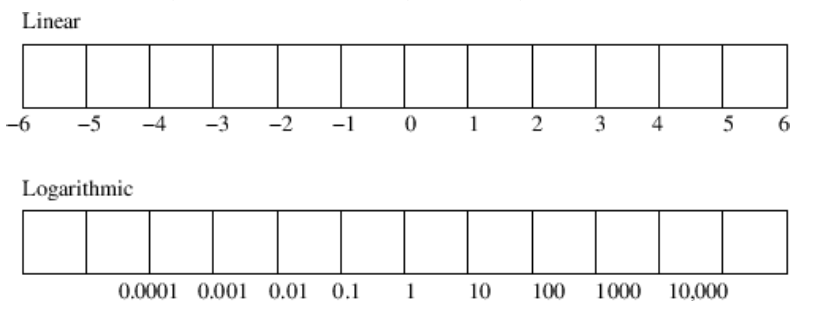
\includegraphics[width=0.93\textwidth]{linear_log_scale.png} \\


\vfill % Pushes the following text to the bottom of the page
\flushleft
\end{center}

% ------------------------- PAGE 6 ------------------------

% Header Section
\newpage
\noindent Year 12 Mathematical Methods \hfill Term 1

\subsection*{Decibel Scale}

The decibel scale is a type of logarithmic scale that is used to describe sound intensity. Because of the way that the ear works, the difference in intensity (measured in watts per metre square) between two sounds might be orders of magnitude apart whilst sounding quite similar. Hence, the decibel scale compares sound intensity in a way that is more relatable for practical use.
\vspace{10pt}

The scale is given below, where \( L \) represents the level in decibels (dB) that corresponds to a given sound wave with intensity \( I \) in \( W/m^2 \). \( I_0 \) is the reference intensity and corresponds to 0 dB, which is the intensity of a 1000 Hz wave at the threshold of hearing (\( \sim 10^{-12} W/m^2 \)).

\[
L = 10 \log_{10} \left( \frac{I}{I_0} \right)
\]

The table below shows some examples of different sounds, their associated level decibels, and their linear intensity.

\begin{center}
\begin{tabular}{|c|c|l|}
\hline
\textbf{Decibels (dB)} & \textbf{Intensity} (\( W/m^2 \)) & \textbf{Example of sound} \\
\hline
130 & \( 10 \) & artillery fire at close proximity (threshold of pain) \\
120 & \( 1 \) & amplified rock music; near jet engine \\
110 & \( 10^{-1} \) & loud orchestral music, in audience \\
100 & \( 10^{-2} \) & electric saw \\
90 & \( 10^{-3} \) & bus or truck interior \\
80 & \( 10^{-4} \) & automobile interior \\
70 & \( 10^{-5} \) & average street noise; loud telephone bell \\
60 & \( 10^{-6} \) & normal conversation; business office \\
\hline
\end{tabular}
\end{center}

\subsection*{Richter Scale}

The Richter scale is a type of logarithmic scale that is used to measure an earthquake's magnitude. The scale is based off of the amplitude of the earthquake's largest seismic wave (the vibration caused by the earthquake).

The scale is given below, where \( M \) is the magnitude of the earthquake, \( I \) is the amplitude, or intensity of the seismic wave, and \( I_N \) is the comparison intensity. The comparison intensity is calculated depending on a range of factors.

\[ 
  M = \log_{10}\left(\frac{I}{I_N}\right) 
\]


\vfill % Pushes the following text to the bottom of the page
\flushleft

% ------------------------- PAGE 7 ------------------------

\newpage % Starts a new page

% Header Section
\noindent Year 12 Mathematical Methods \hfill Term 1


\subsection*{SOLVING EQUATIONS INVOLVING INDICES}

\noindent Here is a quick recap of the index laws:
\begin{itemize}
    \item \(a^m \cdot a^n = a^{m+n}\)
    \item \(\frac{a^m}{a^n} = a^{m-n}\)
    \item \((a^m)^n = a^{mn}\)
    \item \((ab)^m = a^m \cdot b^m\)
    \item \(\left(\frac{a}{b}\right)^m = \frac{a^m}{b^m}\)
    \item \(a^{\frac{m}{n}} = \sqrt[n]{a^m}\)
\end{itemize}

\noindent Some other important properties are as follows:
\begin{itemize}
    \item \(a^0 = 1\)
    \item \(a^{-x} = \frac{1}{a^x}\)
    \item \(\left(\frac{a}{b}\right)^{-m} = \left(\frac{b}{a}\right)^m\)
    \item \(a^{\frac{m}{n}} = \sqrt[n]{a^m}\)
\end{itemize}

\noindent With these laws and properties, you should have everything you need to start solving equations involving indices.

\subsection*{Example:}
\noindent Solve for \(x\) in the equation \(10^x = 50\) 

\noindent Convert to logarithm form and calculate:
\[x = \log_{10}(50) = 1.70\] 

\subsection*{Question:}
% Question 11
\noindent 11. \(2^x = 32\) 
\vspace{10mm} % Adds space for the answer
\noindent \makebox[\linewidth]{\dotfill} % This creates a dotted line
\vspace{10mm}
\noindent \makebox[\linewidth]{\dotfill}
\vspace{10mm}
\noindent \makebox[\linewidth]{\dotfill}

\vfill % Pushes the following text to the bottom of the page
\flushleft

% ------------------------- PAGE 8 ------------------------

\newpage % Starts a new page

% Header Section
\noindent Year 12 Mathematical Methods \hfill Term 1


% Questions continue
\vspace{10mm}\noindent 12. \(3^x = 81\)
\vspace{10mm} % Adds space for the answer
\noindent \makebox[\linewidth]{\dotfill} % This creates a dotted line
\vspace{10mm}
\noindent \makebox[\linewidth]{\dotfill}
\vspace{10mm}
\noindent \makebox[\linewidth]{\dotfill}

\noindent 13. \(343x^3 = 7\)
\vspace{10mm} % Adds space for the answer
\noindent \makebox[\linewidth]{\dotfill} % This creates a dotted line
\vspace{10mm}
\noindent \makebox[\linewidth]{\dotfill}
\vspace{10mm}
\noindent \makebox[\linewidth]{\dotfill}

\noindent Convert the following to logarithmic form with \(x\) as the subject:

\vspace{5mm} % Adds space for the answer
\noindent 14. \((ab)^{\frac{x}{z}} = z\)
\vspace{10mm} % Adds space for the answer
\noindent \makebox[\linewidth]{\dotfill} % This creates a dotted line
\vspace{10mm}
\noindent \makebox[\linewidth]{\dotfill}
\vspace{10mm}
\noindent \makebox[\linewidth]{\dotfill}

\noindent 15. \(n \left(\frac{a}{b}\right)^{\sqrt{x}} = m\)
\vspace{10mm} % Adds space for the answer
\noindent \makebox[\linewidth]{\dotfill} % This creates a dotted line
\vspace{10mm}
\noindent \makebox[\linewidth]{\dotfill}
\vspace{10mm}
\noindent \makebox[\linewidth]{\dotfill}

\vfill % Pushes the following text to the bottom of the page
\flushleft


% ------------------------- PAGE 9 ------------------------
\newpage % Starts a new page

% Header Section
\noindent Year 12 Mathematical Methods \hfill Term 1

% Questions continue
\vspace{10mm}\noindent 16. Simplify \(\log(2) - (\log(10) + 2\log(4))\)\vspace{10mm} 
\vspace{10mm} % Adds space for the answer
\noindent \makebox[\linewidth]{\dotfill} % This creates a dotted line
\vspace{10mm}
\noindent \makebox[\linewidth]{\dotfill}
\vspace{10mm}
\noindent \makebox[\linewidth]{\dotfill}

\noindent 17. Simplify \(\log(15) + \log(10)\)\vspace{10mm}
\vspace{10mm} % Adds space for the answer
\noindent \makebox[\linewidth]{\dotfill} % This creates a dotted line
\vspace{10mm}
\noindent \makebox[\linewidth]{\dotfill}
\vspace{10mm}
\noindent \makebox[\linewidth]{\dotfill}

\noindent 18. Write \(\log_a \left(\frac{1}{a^{\frac{1}{2}}}\right) + 3\log_a \sqrt{x}\) in terms of \(\log_a(x)\)\vspace{10mm}
\vspace{10mm} % Adds space for the answer
\noindent \makebox[\linewidth]{\dotfill} % This creates a dotted line
\vspace{10mm}
\noindent \makebox[\linewidth]{\dotfill}
\vspace{10mm}
\noindent \makebox[\linewidth]{\dotfill}

\vfill % Pushes the following text to the bottom of the page
\flushleft
% ------------------------- PAGE 10 ------------------------
\newpage % Starts a new page

% Header Section
\noindent Year 12 Mathematical Methods \hfill Term 1

% Questions continue
\vspace{10mm}\noindent 19. Write \(\log_a \left(\frac{x^2}{\sqrt{y}}\right)\) as a summation of \(\log_a(x)\), \(\log_a(y)\), and \(\log_a(z)\)\vspace{10mm}
\vspace{10mm} % Adds space for the answer
\noindent \makebox[\linewidth]{\dotfill} % This creates a dotted line
\vspace{10mm}
\noindent \makebox[\linewidth]{\dotfill}
\vspace{10mm}
\noindent \makebox[\linewidth]{\dotfill}

% Questions continue
\noindent 20. Given that \( a^3 = 15 \), find \( a^6 \).\vspace{10mm}
\vspace{10mm} % Adds space for the answer
\noindent \makebox[\linewidth]{\dotfill} % This creates a dotted line
\vspace{10mm}
\noindent \makebox[\linewidth]{\dotfill}
\vspace{10mm}
\noindent \makebox[\linewidth]{\dotfill}

\noindent 21. Given that \( a^5 = 34 \), find \( a^3 \).\vspace{10mm}
\vspace{10mm} % Adds space for the answer
\noindent \makebox[\linewidth]{\dotfill} % This creates a dotted line
\vspace{10mm}
\noindent \makebox[\linewidth]{\dotfill}
\vspace{10mm}
\noindent \makebox[\linewidth]{\dotfill}

\vfill % Pushes the following text to the bottom of the page
\flushleft

% ------------------------- NEXT QUESTION PAGE ------------------------
\newpage % Starts a new page

% Header Section
\noindent Year 12 Mathematical Methods \hfill Term 1

% Questions continue
\vspace{5mm}\noindent 23. Given that \( a^6 = 50 \), find \( (6a)^3 \).\vspace{10mm}
\vspace{10mm} % Adds space for the answer
\noindent \makebox[\linewidth]{\dotfill} % This creates a dotted line
\vspace{10mm}
\noindent \makebox[\linewidth]{\dotfill}
\vspace{10mm}
\noindent \makebox[\linewidth]{\dotfill}

\noindent 24. Solve \( 2^{x+6} = 16 \)\vspace{10mm}
\vspace{10mm} % Adds space for the answer
\noindent \makebox[\linewidth]{\dotfill} % This creates a dotted line
\vspace{10mm}
\noindent \makebox[\linewidth]{\dotfill}
\vspace{10mm}
\noindent \makebox[\linewidth]{\dotfill}

\noindent 25. Solve \( \left(\frac{1}{10}\right)^{5x} = 10 \)\vspace{10mm}
\vspace{10mm} % Adds space for the answer
\noindent \makebox[\linewidth]{\dotfill} % This creates a dotted line
\vspace{10mm}
\noindent \makebox[\linewidth]{\dotfill}
\vspace{10mm}
\noindent \makebox[\linewidth]{\dotfill}

\noindent 26. Solve \( 8^{1/3}\log_{8}(64x^3) = 8 \)\vspace{10mm}
\vspace{10mm} % Adds space for the answer
\noindent \makebox[\linewidth]{\dotfill} % This creates a dotted line
\vspace{10mm}
\noindent \makebox[\linewidth]{\dotfill}
\vspace{10mm}
\noindent \makebox[\linewidth]{\dotfill}

\vfill % Pushes the following text to the bottom of the page
\flushleft


% ------------------------- HOMEWORK QUESTIONS PAGE ------------------------

% Header Section
\noindent \textbf{HOMEWORK QUESTIONS}

\noindent Solve the following:

\vspace{5mm}\noindent 1. \( 2^x > 12 \)\vspace{5mm}
\vspace{10mm} % Adds space for the answer
\noindent \makebox[\linewidth]{\dotfill} % This creates a dotted line
\vspace{10mm}
\noindent \makebox[\linewidth]{\dotfill}
\vspace{10mm}
\noindent \makebox[\linewidth]{\dotfill}

\vspace{5mm}\noindent 2. \( 3^{x-2} > 27 \)\vspace{5mm}
\vspace{10mm} % Adds space for the answer
\noindent \makebox[\linewidth]{\dotfill} % This creates a dotted line
\vspace{10mm}
\noindent \makebox[\linewidth]{\dotfill}
\vspace{10mm}
\noindent \makebox[\linewidth]{\dotfill}

\vspace{5mm}\noindent 3. \( 2 \leq 2^x \leq 128 \)\vspace{5mm}
\vspace{10mm} % Adds space for the answer
\noindent \makebox[\linewidth]{\dotfill} % This creates a dotted line
\vspace{10mm}
\noindent \makebox[\linewidth]{\dotfill}
\vspace{10mm}
\noindent \makebox[\linewidth]{\dotfill}

\vspace{5mm}\noindent 4. \( 7 \cdot 3^{-x} \leq 60 \)\vspace{5mm}
\vspace{10mm} % Adds space for the answer
\noindent \makebox[\linewidth]{\dotfill} % This creates a dotted line
\vspace{10mm}
\noindent \makebox[\linewidth]{\dotfill}
\vspace{10mm}
\noindent \makebox[\linewidth]{\dotfill}

% ------------------------- ADDITIONAL QUESTIONS PAGE ------------------------
\newpage % Starts a new page

% Questions continue
\noindent \textbf{HOMEWORK QUESTIONS}

\vspace{5mm}\noindent 5. \( \log_x(81) = \frac{2x}{2^3} \)\vspace{5mm}
\vspace{10mm} % Adds space for the answer
\noindent \makebox[\linewidth]{\dotfill} % This creates a dotted line
\vspace{10mm}
\noindent \makebox[\linewidth]{\dotfill}
\vspace{10mm}
\noindent \makebox[\linewidth]{\dotfill}

\noindent 6. By solving \( 2^x < 10^{20} \), find how many positive integer powers of 2 are less than \( 10^{20} \).\vspace{5mm}
\vspace{10mm} % Adds space for the answer
\noindent \makebox[\linewidth]{\dotfill} % This creates a dotted line
\vspace{10mm}
\noindent \makebox[\linewidth]{\dotfill}
\vspace{10mm}
\noindent \makebox[\linewidth]{\dotfill}

% Questions continue
\vspace{5mm}\noindent 7. By solving \( 10^5 < 5^x < 10^{30} \), find how many integer powers of 5 are between \( 10^5 \) and \( 10^{30} \).\vspace{5mm}
\vspace{10mm} % Adds space for the answer
\noindent \makebox[\linewidth]{\dotfill} % This creates a dotted line
\vspace{10mm}
\noindent \makebox[\linewidth]{\dotfill}
\vspace{10mm}
\noindent \makebox[\linewidth]{\dotfill}

\noindent 8. Explain why the majority of the logarithmic scales we looked at used a base of 10.\vspace{5mm}
\vspace{10mm} % Adds space for the answer
\noindent \makebox[\linewidth]{\dotfill} % This creates a dotted line
\vspace{10mm}
\noindent \makebox[\linewidth]{\dotfill}
\vspace{10mm}
\noindent \makebox[\linewidth]{\dotfill}


\end{document}
